%%%%%%%%%%%%%%%%%%%%%%%%%%%%%%%%%%%%%%%%%%%%%%%%%%%
%% P3: Phenomenology of Particle Physics                         
%%
%% Author:  André Rubbia                   		 
%%
%% Figure 21.9 Improved setup at the Savannah River power plant.
%%
%% This work is licensed under the Creative Commons Attribution 4.0 International License. 
%% To view a copy of this license, visit http://creativecommons.org/licenses/by/4.0/ or 
%% send a letter to Creative Commons, PO Box 1866, Mountain View, CA 94042, USA.
%%
%%%%%%%%%%%%%%%%%%%%%%%%%%%%%%%%%%%%%%%%%%%%%%%%%%%

\documentclass[a4paper,10pt]{article}

\usepackage[T1]{fontenc}
\usepackage[utf8]{inputenc}
\usepackage{lmodern}
\usepackage[labelfont=bf]{caption}
\usepackage{upgreek}

\usepackage{tikz}
\usetikzlibrary{patterns}
\usetikzlibrary{decorations.pathmorphing}
\usetikzlibrary{decorations.markings}
\usetikzlibrary{arrows}
\usetikzlibrary{svg.path}
\usetikzlibrary{shapes}
\usetikzlibrary{arrows.meta}
% define the arrow style
\tikzset{
    arrow/.style={
        decoration={
            markings,
            mark=at position .5 with {
                \arrow[#1, scale=1.5]{latex}
            }
        },
        postaction={decorate},
    }
}
\tikzset{
    arrow flipped/.style={
        decoration={
            markings,
            mark=at position .5 with {
                \arrow[#1, scale=1.5]{latex reversed}
            }
        },
        postaction={decorate},
    }
}
\usepackage{pgfplots}
\pgfplotsset{compat=1.17}
\usepgfplotslibrary{ternary}
\usepgfplotslibrary{fillbetween}
\usepgfplotslibrary{external}

\def\d{\mathrm{d}}
\setlength{\oddsidemargin}{-1.0cm}
\setlength{\evensidemargin}{-1.0cm}
\setlength{\textheight}{25cm}
\setlength{\textwidth}{18cm}

\begin{document}

%%%%%%%%%%%%%%%%   FIGURE  %%%%%%%%%%%%%%%%%%%%%%%%%%%%%%
\begin{figure}[htb]
\centering
    \begin{tikzpicture}[scale=0.75]
	\foreach \x in {0, 6} {
		\foreach \y in {0, 2.5, 5}
		  {\begin{scope}[shift={(\x,\y)}]
		      \draw[thick] (0,0) rectangle +(5,1.5);
		  \end{scope}};
		    \draw[thick, fill,color=yellow] (\x,1.75) rectangle +(5,0.5);
		    \draw[thick, fill,color=yellow] (\x,4.25) rectangle +(5,0.5);
		    \draw[blue,fill] (\x + 2,4.5) circle (2pt);
	    };
	    \draw[dashed] (1,7) node [above] {$\bar \nu$} -- (2,4.5);
	    \draw[red] (2,4.5) -- +(0.5,-0.2);
	    \draw[blue] (6 + 2,4.5) -- +(0.1,0.1) -- +(-0.2,0) -- +(-0.3,-0.1) -- +(-0.4,0.15) -- +(-0.5,-0.1) -- +(-0.6,0.1);
	    \draw[red,->, decorate, decoration=snake,very thick] (2.5,4.3)  -- +(1.5,1.5) node[right] {$\gamma$};
	    \draw[red,->, decorate, decoration=snake,very thick] (2.5,4.3)  -- +(-1.5,-1.5) node[left] {$\gamma$};
	    \draw[blue,->, decorate, decoration=snake,very thick] (7.4,4.6)  -- +(0.5,1.5) node[right] {$\gamma$};
	    \draw[blue,->, decorate, decoration=snake,very thick] (7.4,4.6)  -- +(-0.5,-1.5) node[right] {$\gamma$};
	    \draw[blue,->, decorate, decoration=snake,very thick] (7.4,4.6)  -- +(0.5,-1.5) node[right] {$\gamma$};
	    \node[left] at (-0.5,4.5) { Target $\mathrm{H_2O + CdCl_2}$ tank A};
	    \node[left] at (-0.5,2.) { Target $\mathrm{H_2O + CdCl_2}$ tank B};
	    \node[left] at (-0.5,5.75) { Liquid Scintillator Detector I};
	    \node[left] at (-0.5,3.25) { Liquid Scintillator Detector II};
	    \node[left] at (-0.5,0.75) { Liquid Scintillator Detector III};
	    \draw[-, thick] (-1,-1) node[left] {Signal I} -- +(4,0) -- +(4,0.3) -- +(4.25,0) -- +(9,0) -- +(9,0.65) -- +(9.25,0) -- +(11,0) ;
	    \draw[-, thick] (-1,-2) node[left] {Signal II} -- +(4,0) -- +(4,0.3) -- +(4.25,0) -- +(9,0) -- +(9,0.9) -- +(9.25,0) -- +(11,0) ;
	    \draw[-, thick] (-1,-3) node[left] {Signal III} -- +(11,0) ;
	    \draw[<->, very thick] (-1+4,-2.5)  -- +(5,0) node[right] {$\Delta t\approx \mu$s};
	    \node[red,left] at (2.75,-1.5) {$e^+$};
	    \node[blue,left] at (7.75,-1.5) {$n$};
  \end{tikzpicture}
\caption{Improved setup at the Savannah River power plant with a separation between
target (H$_2$O + CdCl$_2$) and detector consisting of liquid scintillator: (left) the two gammas from the
annihilation of the positron are detected in the external tanks filled with liquid scintillator (I and II in the picture);
(right) after diffusion in the target, the neutron is captured on Cd, which releases gammas that
are also detected in the detectors.
}
\end{figure}
%
%%%%%%%%%%%%%%%%   END FIGURE  %%%%%%%%%%%%%%%%%%%%%%%%%%%%%%
%
\end{document}
